\documentclass[12pt]{article}
\title{Understanding the Slope Foraging Problem}
\author{Mostafa Rizk}

\usepackage{graphicx}
\usepackage{subfig}
\usepackage[margin=1.5in]{geometry}
\usepackage{fancyhdr}
\usepackage{url}
\usepackage{tabu}
\usepackage[colorinlistoftodos,prependcaption,textsize=tiny]{todonotes}
\usepackage[toc,page]{appendix}

\fancyhead{}
\fancyfoot{}
\fancyfoot[R]{\thepage}

\pagestyle{fancy}
\begin{document}
\maketitle
\tableofcontents

\section{Executive Summary}

\section{Introduction}

We're interested in evolving multi-agent cooperation.
Use Slope Foraging as test bed.
Insights gained from this relatively simple setup can hopefully be applied to other tasks that share attributes with this one.
Want to place this problem in the context of known ones in the literature.
How difficult is it?
We use rwg benchmarking to compare it to known tasks.
We then discuss Stag Hunt games.

\section{Task Description}\label{task_description}

The task is modelled off the foraging behaviour of the Atta Leafcutter ant, as in Ferrante et al \cite{ferrante:PLOS_CB:2015} and Pini et al \cite{pini:ICSI:2012, pini:Swarm_Intelligence:2011}.
In nature, the ants cut leaves from a tree and take them to their nest. 
Sometimes the ants partition the task. 
When they do so, some ants are droppers, who cut leaves and let them fall, while other ants are collectors who collect fallen leaves from the base of the tree and take them to the nest.
This partitioned approach is advantageous because gravity transports leaves faster than ants can.
Rather than every ant climbing up the tree, cutting a leaf and bringing it to the nest, when they partition the ants are able to transport more leaves in the same time-span while consuming less energy.\\

We model this scenario similarly to Ferrante et al \cite{ferrante:PLOS_CB:2015}, with a slope in place of the tree trunk. 
Pini et al use a slightly different implementation where the resources can be transported via a long corridor or a booth with a wait time \cite{pini:ICSI:2012, pini:Swarm_Intelligence:2011}. 
This approach may be useful for comparison at a later stage of the research.
Much like the ants, agents transport resources from the source to the nest.
An agent on a team can use a generalist strategy where it acts individually, going up and down the slope to retrieve resources.
An agent can also use a specialist strategy. 
As a specialist it can either be a dropper, going up the slope once and dropping things from the nest, or it can be a collector and gather the resources that accumulate at the base of the slope, called the cache.
Much like real robots that deplete their battery and ants that deplete their energy stores, there is a cost to moving and it is compounded when going up the slope. 
Teams that use complementary specialist strategies pay a smaller energy cost as well as time cost, since resources slide down faster than they can be carried. 
Preliminary analysis with hard-coded agents verifies that specialist teams gain higher overall reward than generalist teams (Table \ref{tab:hardcoded}.\\

More formally, you have a team of $n_{agents}$ agents. 
They are placed in a rectangular arena that is $l$ tiles long and $w$ tiles wide, illustrated in Figure \ref{fig:arena} and Figure \ref{fig:arena_2}. 
The arena is divided into four sections $l= l_{nest} + l_{cache} + l_{slope} + l_{source}$.
Each episode is composed of a number of finite time-steps $t=0, .... T$. 
Since 3D physics is computationally expensive we use a 2D environment to expedite our experiments as the focus of our research is on the evolutionary process and team dynamics rather than the robotic element.
We also use a discrete scenario, as opposed to a continuous one for further simplicity.
To simulate the presence of gravity, resources move when on the slope, at a speed greater than the agents are capable of.
The high sliding speed creates evolutionary pressure for the team to specialise.
Agents travel at speed $s_{agent}$ and resources slide when placed on the slope with a speed of $s_{resource}$ 
Additionally agents pay costs for moving.
This simulates the presence of a battery, with energy expenditure varying depending on where the agent is moving.
There is a base cost to moving $c$ paid by the agent for moving in any direction.
The base cost is multiplied by different factors for moving up the slope ($f_{up}$) down the slope ($f_{down}$) and moving while carrying a resource ($f_{carry}$). 
An agent moving sideways on the slope pays the same cost as one moving on a non-slope area in any direction.
An agent moving one tile up the slope at time step $t=0$ while carrying a resource, for example, pays a cost of $C_{0} = f_{up} \cdot f_{carry} \cdot c$ .
There are $n_{resources}$ resources at the source, initially.
Every time a resource is removed from the source, another one appears at the source so there are always at least $n_{resources}$.
Each resource retrieved provides all team members a reward of $R$.
The values we chose for these parameters can be found in the appendix\\

Fitness can be calculated for the team or for an individual depending on the level of selection.
When calculating fitness for a team of agents, the fitness function is as follows:\\ 
\\
$F = \sum_{t=1}^{T} \sum_{i}^{n_{agents}} (R_{ti} - C_{ti}) $\\
\\
That is, for each agent, at each time step, we calculate the reward it received at that time step (whether from retrieving a resource itself or from another agent retrieving a resource) and we subtract the cost it individually paid at that time step. 
We then take the summation of this calculation for all agents over all time steps in the simulation.
The reward and cost for an agent $i$ at time step $t$ can be computed as shown here:\\
\\
$
R_{ti} = R \cdot r_{t}
$\\
\\
where $r_t$ is the total number of resources retrieved by all agents at time $t$
\\
\\
\\
$
C_{ti} = \left\{
        \begin{array}{ll}
            c & \quad not on slope or moved sideways on slope\\
            c \cdot f_{up} & \quad up slope\\
            c \cdot f_{down} & \quad down slope\\
            c \cdot f_{carry} & \quad not on slope or moved sideways on slope while carrying\\
            c \cdot f_{carry} \cdot f_{up} & \quad up slope while carrying \\
            c \cdot f_{carry} \cdot f_{down} & \quad down slope while carrying\\
        \end{array}
    \right.
$
\\
\\
When calculating fitness for an individual agent, the fitness function is as follows:\\
\\
$F = \sum_{t=1}^{T} (R_{ti} - C_{ti}) $
\\
\\
Example: Agent 1 incurs -200 retrieving resource. 
Agent 2 incurs -100 wandering around cache. 
Agent 1 score= 1000 - 200. 
Agent 2 score = 1000 - 100.
Team selection: team score = agent 1 score + agent 2 score = 800 + 900 = 1700
Individual selection: agent 1 score = 800, agent 2 score = 900. 
In team selection, each team is compared to other teams. 
In individual selection, the highest scoring individual is selected. 

\begin{figure}
	\centering
	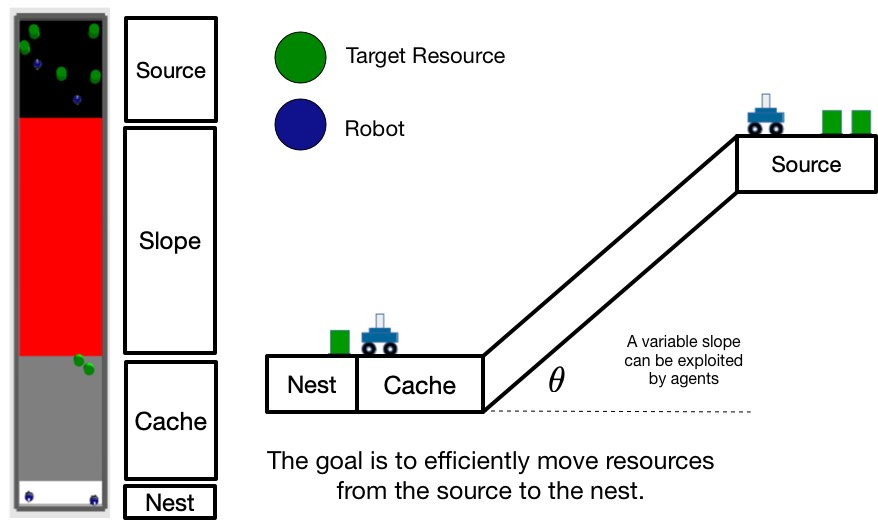
\includegraphics[width=\textwidth]{arena.jpg}
	\caption{Arena Layout}
	\label{fig:arena}
\end{figure}

\begin{figure}
	\centering
	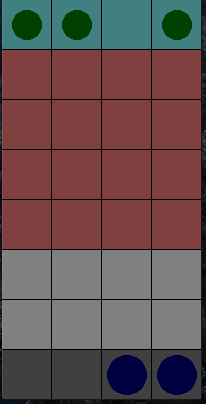
\includegraphics[width=0.3\textwidth]{arena_layout.png}
	\caption{Arena Screenshot}
	\label{fig:arena_2}
\end{figure}

\subsection{Observations and Actions}\label{observation_space}

Agents have a sensing range that indicates how many tiles around them they can observe. 
A sensing range of 0 means an agent can just observe the current tile it is on. 
A range of 1 means it can observe a square centred  on its location that extends 1 tile in each direction (9 tiles total including current tile). 
A range of 2 means it can observe a square extending 2 tiles in each direction (25 tiles total). 
And so on.
We assume our agent represents a robot with only local sensing capabilities and use a sensing range of 1, which has the added benefit of reducing computation.
For each tile in its sensing range, an agent observes a onehotencoded 4-bit vector. 
The values it reads denote the following: Blank= 1000, Agent = 0100, Resource = 0010, Wall = 0001.
Tiles are read row by row from top left to bottom right. 
The next part of an agent's observation is a 4-bit vector denoting which part of the arena it is on, similar to a real robot with a ground sensor that can detect the unique colour of each area.
The values of this vector can be as follows: Nest = 1000, Cache = 0100, Slope = 0010, Source = 0001
The final part of an agent's observation is 1-bit for resource possession. 
The values can be as follows: Has resource = 1, Doesn’t have resource = 0
The total length of the observation vector is 9x4 + 4 + 1= 41 bits.\\

An agent can perform 6 possible actions, represented by the following values: Forward = 0, Backward = 1, Left = 2, Right = 3, Pick-up = 4, Drop = 5.
We use a recurrent neural network to choose actions based on the observed state.
Since many of the positions in the environment will produce the same observation, a recurrent neural network gives the agent a simple form of memory, preventing it from getting "stuck" in infinite state transition loops.
The default network has 41 inputs, 1 bias input and 6 recurrent inputs (one for each of the 6 outputs). 
There is no hidden layer, just a 6-neuron output layer. 
This makes for a total of (41+1+6)x6 = 288 weights. 
The output layer uses a linear activation function.

\section{Experimental Methods}

We use the same setup as Oller et al \cite{oller:AAMAS:2020}.
We use 3 different architectures: a feedforward neural network (FFNN) with no hidden layers, one with 1 hidden layer composed of 4 hidden units and one with 2 hidden layers also composed of 4 hidden units.
We ran experiments with and without a bias neuron and found no noticeable difference. We include the no- bias plots.
All networks use tanh activation.
For each architecture, we sample 10,000 genomes, where each genome contains weights for two neural networks, one for each agent on the team.
For each sampled genome, we do 20 runs of the simulation (i.e. 20 episodes). 

\section{Results}

\begin{figure}
	\centering
	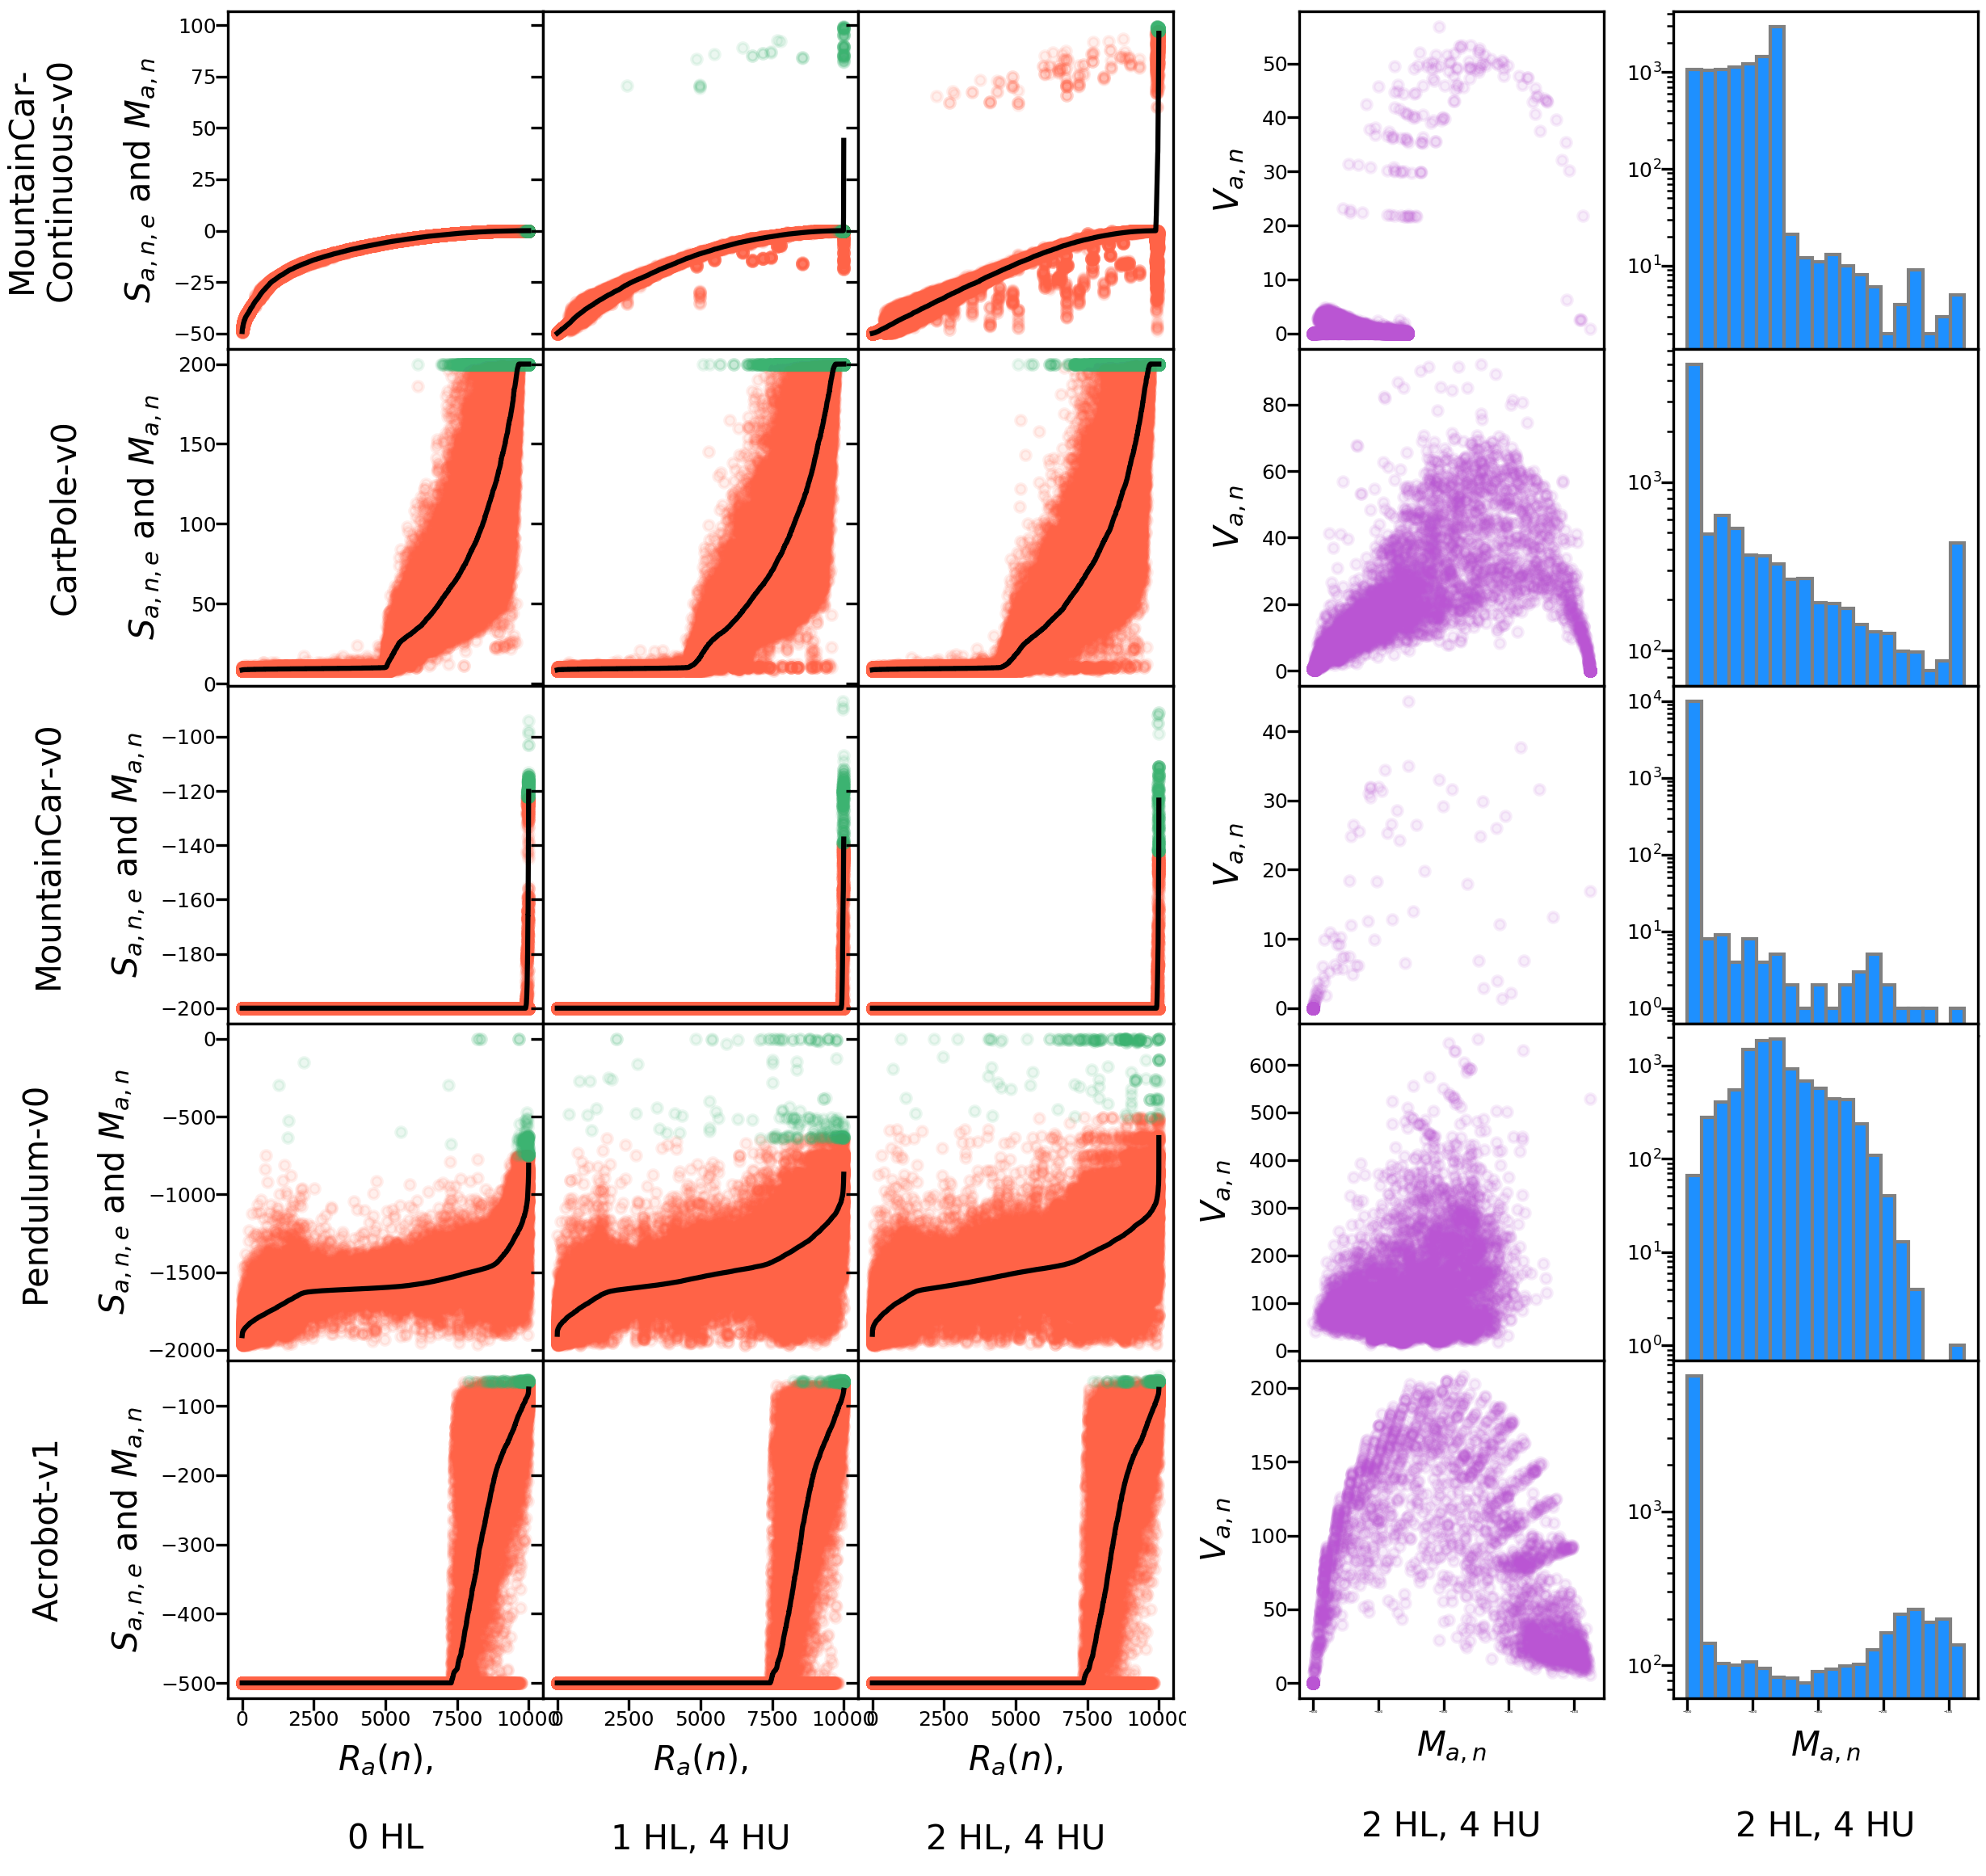
\includegraphics[width=\textwidth]{plots/oller_plot.png}
	\caption{RWG Analysis of OpenAI Gym Benchmarks}
	\label{fig:oller}
\end{figure}

\begin{figure}[!tbp]
  \centering
  % FFNN no-bias 0HL
  \subfloat{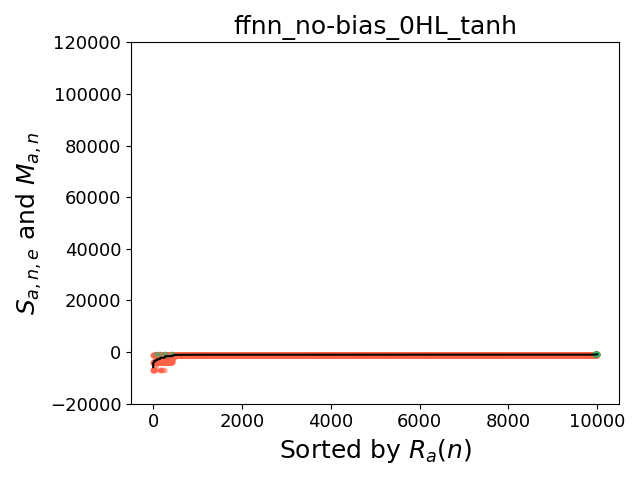
\includegraphics[width=0.3\textwidth]{plots/ffnn_no-bias_0HL_tanh/ffnn_no-bias_0HL_tanh_score_trials_ordered_.png}}
  \hfill
  \subfloat{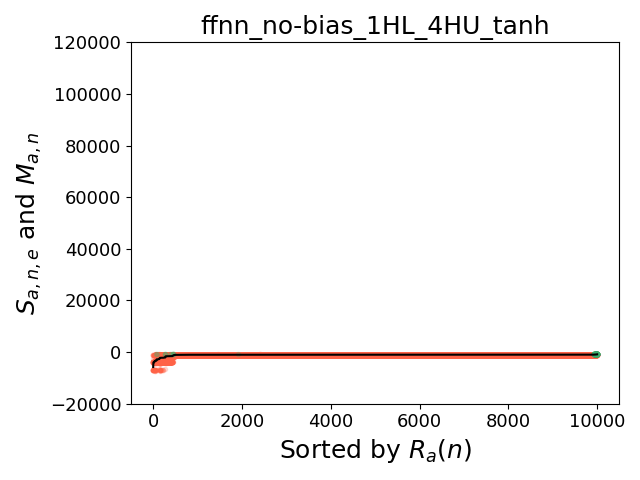
\includegraphics[width=0.3\textwidth]{plots/ffnn_no-bias_1HL_4HU_tanh/ffnn_no-bias_1HL_4HU_tanh_score_trials_ordered_.png}}
  \hfill
  \subfloat{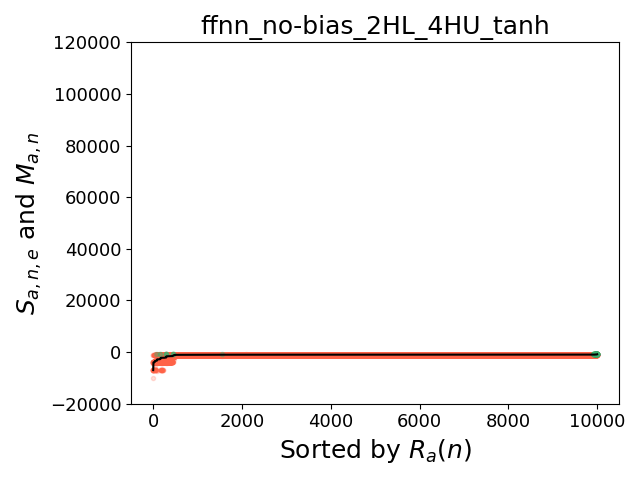
\includegraphics[width=0.3\textwidth]{plots/ffnn_no-bias_2HL_4HU_tanh/ffnn_no-bias_2HL_4HU_tanh_score_trials_ordered_.png}}
  \hfill
  \subfloat{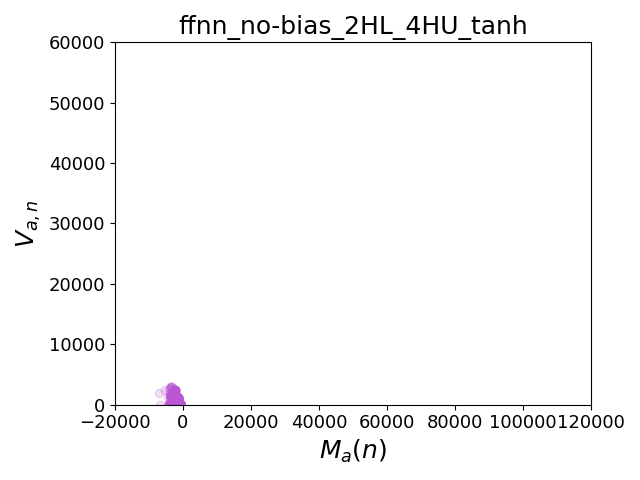
\includegraphics[width=0.3\textwidth]{plots/ffnn_no-bias_2HL_4HU_tanh/ffnn_no-bias_2HL_4HU_tanh_variance_meanscore_.png}}
  \hfill
  \subfloat{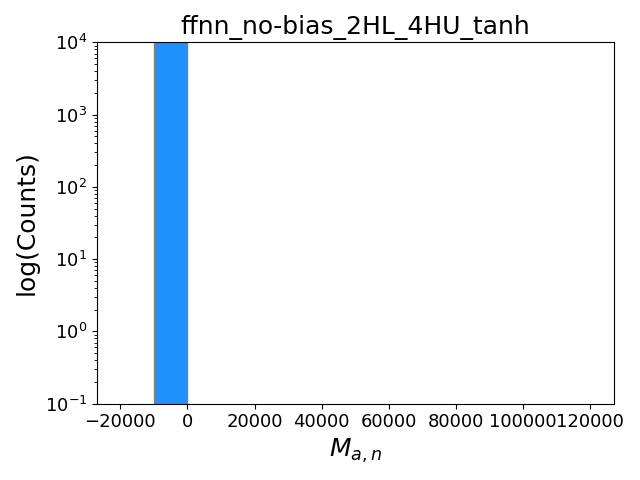
\includegraphics[width=0.3\textwidth]{plots/ffnn_no-bias_2HL_4HU_tanh/ffnn_no-bias_2HL_4HU_tanh_all_scores_log_dist_.png}}
  
  \caption{FFNN no bias}
  \label{fig:ffnn-no-bias}	
\end{figure}

\begin{figure}[!tbp]
  \centering
  % FFNN bias 0HL
  \subfloat{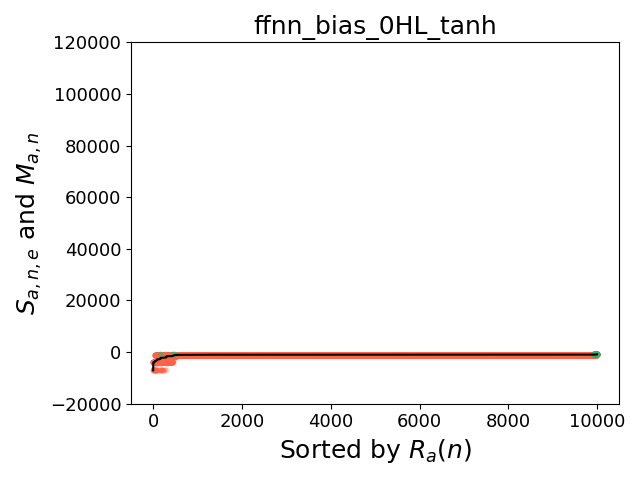
\includegraphics[width=0.3\textwidth]{plots/ffnn_bias_0HL_tanh/ffnn_bias_0HL_tanh_score_trials_ordered_.png}}
  \hfill
  \subfloat{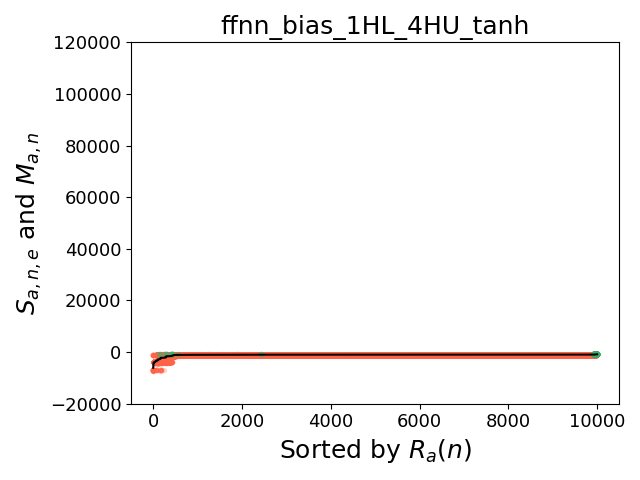
\includegraphics[width=0.3\textwidth]{plots/ffnn_bias_1HL_4HU_tanh/ffnn_bias_1HL_4HU_tanh_score_trials_ordered_.png}}
  \hfill
  \subfloat{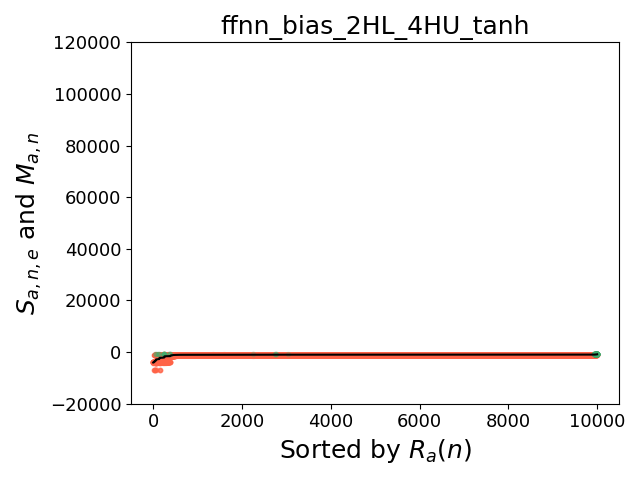
\includegraphics[width=0.3\textwidth]{plots/ffnn_bias_2HL_4HU_tanh/ffnn_bias_2HL_4HU_tanh_score_trials_ordered_.png}}
  \hfill
  \subfloat{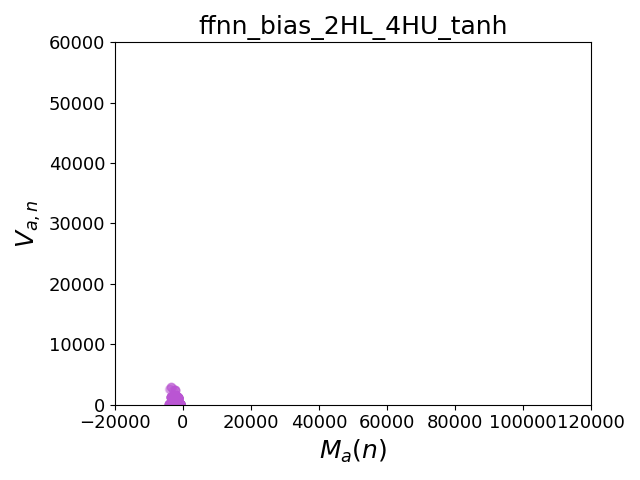
\includegraphics[width=0.3\textwidth]{plots/ffnn_bias_2HL_4HU_tanh/ffnn_bias_2HL_4HU_tanh_variance_meanscore_.png}}
  \hfill
  \subfloat{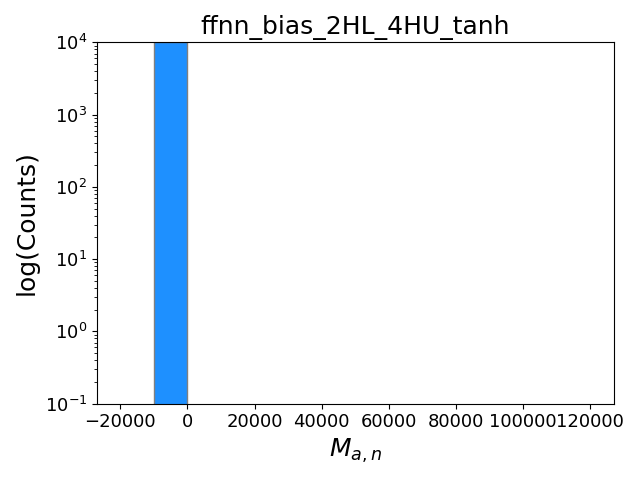
\includegraphics[width=0.3\textwidth]{plots/ffnn_bias_2HL_4HU_tanh/ffnn_bias_2HL_4HU_tanh_all_scores_log_dist_.png}}
  
  \caption{FFNN bias}
  \label{fig:ffnn-bias}	
\end{figure}

\begin{figure}[!tbp]
  \centering
  % RNN no-bias 0HL
  \subfloat{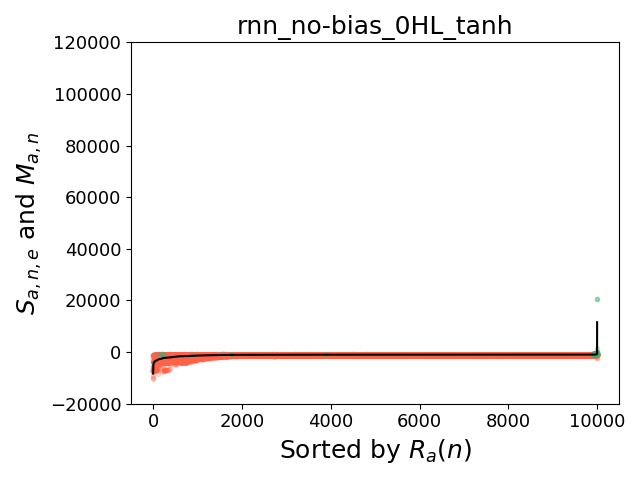
\includegraphics[width=0.3\textwidth]{plots/rnn_no-bias_0HL_tanh/rnn_no-bias_0HL_tanh_score_trials_ordered_.png}}
  \hfill
  \subfloat{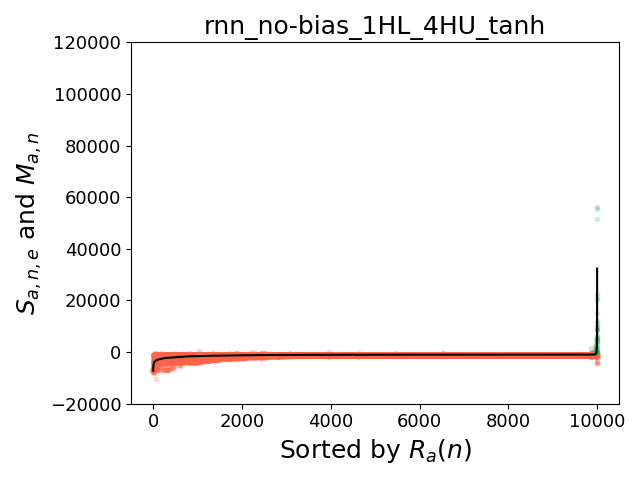
\includegraphics[width=0.3\textwidth]{plots/rnn_no-bias_1HL_4HU_tanh/rnn_no-bias_1HL_4HU_tanh_score_trials_ordered_.png}}
  \hfill
  \subfloat{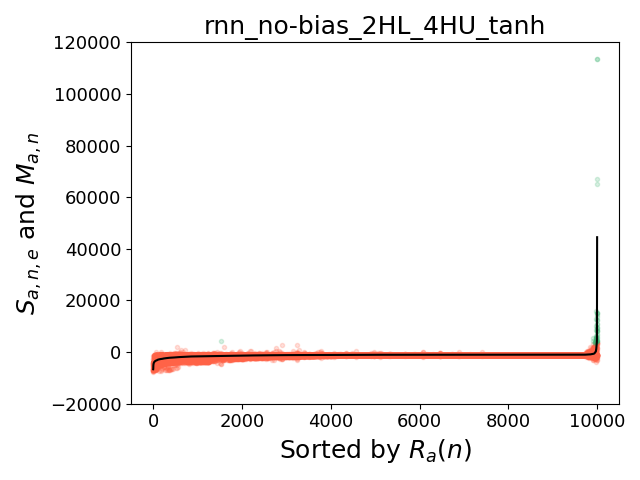
\includegraphics[width=0.3\textwidth]{plots/rnn_no-bias_2HL_4HU_tanh/rnn_no-bias_2HL_4HU_tanh_score_trials_ordered_.png}}
  \hfill
  \subfloat{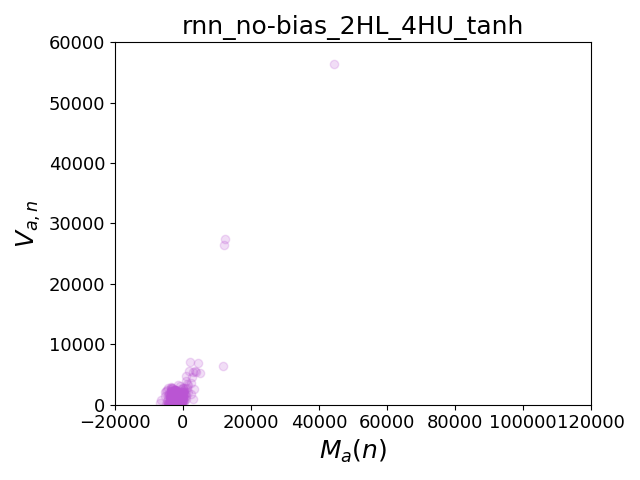
\includegraphics[width=0.3\textwidth]{plots/rnn_no-bias_2HL_4HU_tanh/rnn_no-bias_2HL_4HU_tanh_variance_meanscore_.png}}
  \hfill
  \subfloat{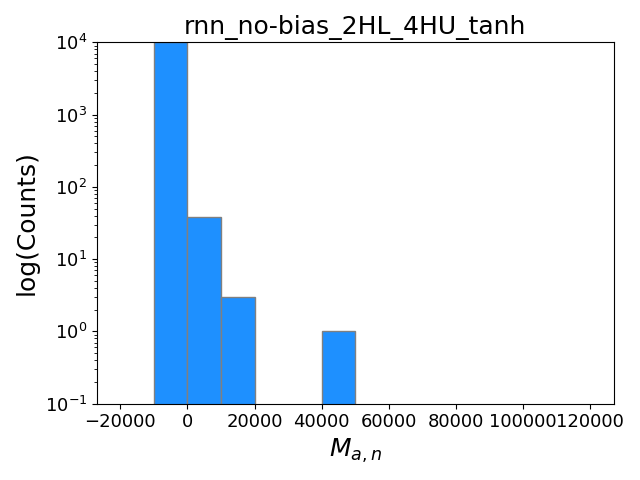
\includegraphics[width=0.3\textwidth]{plots/rnn_no-bias_2HL_4HU_tanh/rnn_no-bias_2HL_4HU_tanh_all_scores_log_dist_.png}}
  
  \caption{RNN no bias}
  \label{fig:rnn-no-bias}	
\end{figure}

\begin{figure}[!tbp]
  \centering
  % RNN bias 0HL
  \subfloat{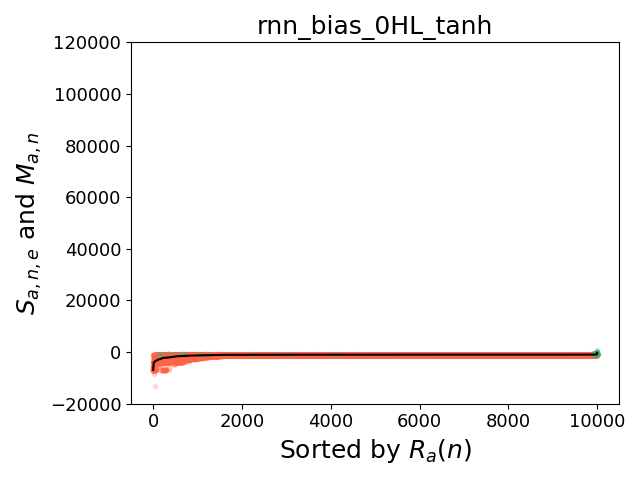
\includegraphics[width=0.3\textwidth]{plots/rnn_bias_0HL_tanh/rnn_bias_0HL_tanh_score_trials_ordered_.png}}
  \hfill
  \subfloat{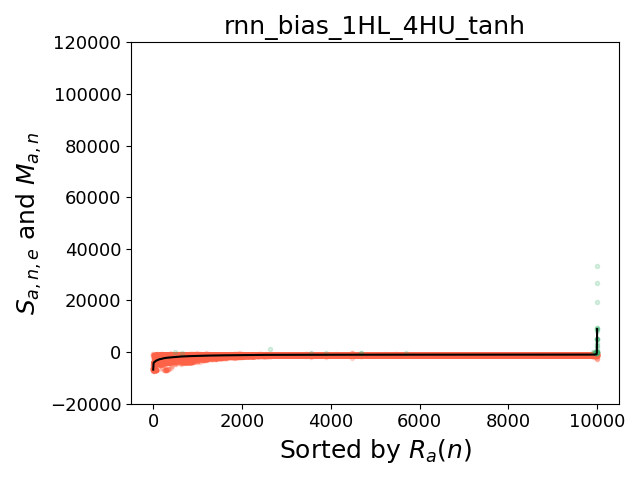
\includegraphics[width=0.3\textwidth]{plots/rnn_bias_1HL_4HU_tanh/rnn_bias_1HL_4HU_tanh_score_trials_ordered_.png}}
  \hfill
  \subfloat{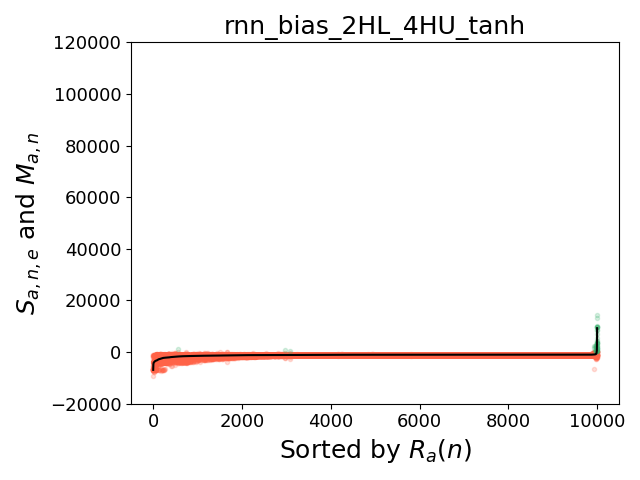
\includegraphics[width=0.3\textwidth]{plots/rnn_bias_2HL_4HU_tanh/rnn_bias_2HL_4HU_tanh_score_trials_ordered_.png}}
  \hfill
  \subfloat{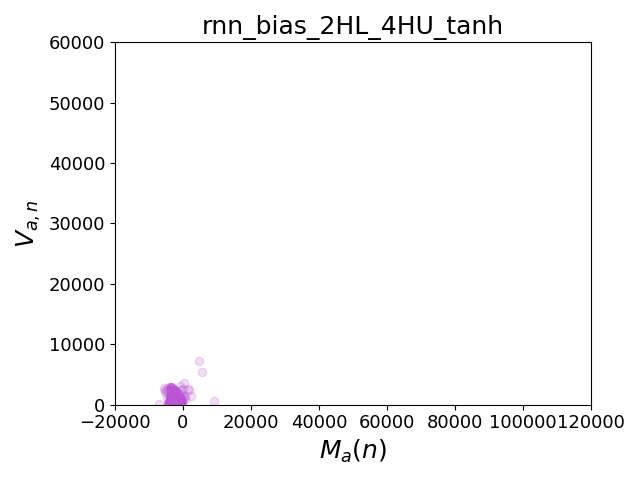
\includegraphics[width=0.3\textwidth]{plots/rnn_bias_2HL_4HU_tanh/rnn_bias_2HL_4HU_tanh_variance_meanscore_.png}}
  \hfill
  \subfloat{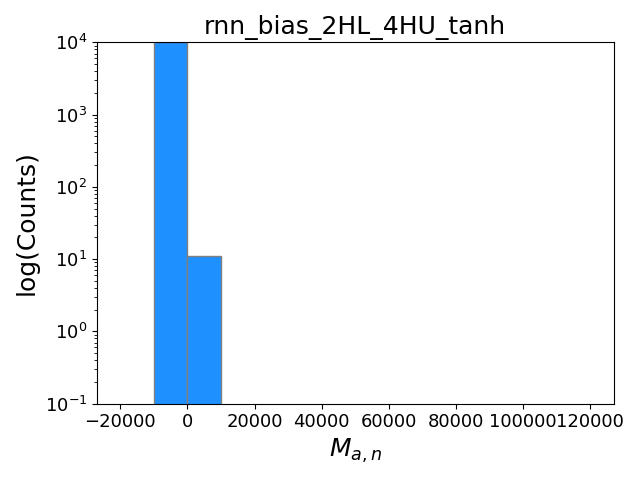
\includegraphics[width=0.3\textwidth]{plots/rnn_bias_2HL_4HU_tanh/rnn_bias_2HL_4HU_tanh_all_scores_log_dist_.png}}
  
  \caption{RNN bias}
  \label{fig:rnn-bias}	
\end{figure}		

Looking at Figure \ref{fig:ffnn-no-bias} and Figure \ref{fig:ffnn-bias} in comparison with the Gym benchmarks in Figure \ref{fig:oller}, we can immediately see that the SlopeForaging task is more difficult than all the standard Gym benchmarks.
The mean score is below zero for all architectures and the distribution histogram for the architecture with two hidden layers shows that all episodes indeed receive negative scores.
This holds whether or not there is a bias neuron.
The same architectures that can successfully solve the Gym benchmarks appear to be insufficient to solve the SlopeForaging problem, indicating that this problem is more difficult than all of Gym's classic control benchmarks.\\

When we observe the failed controllers to see where they go wrong, we see them carrying out repetitive unproductive behaviours or oscillating between states.
For example, an agent at the nest might choose to do a pickup action, despite there being no resource in range.
Since there is no resource in range, the state won't change and the agent's observation will be the same at the next time step and it will do the same action again, repeating itself until the final time step.
Another agent might move forward when in the nest and move backward when in the cache, oscillating between two states until the end of the episode.
Using a FFNN means that if an agent makes a particular observation, they will perform the same action every time they make that observation, meaning it is easy to get stuck like our agents do.
A recurrent neural network (RNN) performs an action based on the observation as well as the last action, so if the observation is the same at time $t$ as it was at $t-1$ then an agent can, in principle, do a different action than the one it did at $t-1$ as that one obviously did not change the state.
Consider the previously mentioned agent that does a pickup action with no resources nearby and makes the same observation at the following time step.
An FFNN-based agent will, by necessity, do that same action again.
An RNN-based agent might do a different action because while the observation is the same, the action it did at $t-1$ may not be.
Of course, there is a chance the network will have the same output for that observation regardless of what the action at $t-1$ was, but the chance of that happening is less than it is for an FFNN, for which it is a certainty.\\

We repeat the experiments with an RNN, with the same combinations of hidden layers and bias.
The RNN achieves much higher scores than the FFNN.
Similar to the FFNN experiments, most samples score poorly, but in contrast, we see in Figures \ref{fig:rnn-no-bias} and \ref{fig:rnn-bias} that top ranked episodes receive non-negative scores, which are only possible if resources are successfully retrieved by the agents.
The mean curve has a spike at the far right, which gets more pronounced as more hidden layers are added.
We also see in the distribution histogram that there are samples whose mean scores fall into higher ranking buckets.
Much like Oller et al \cite{oller:AAMAS:2020} networks with no bias neuron outperform those with a bias neuron.
Most interestingly, we see in Figure \ref{fig:rnn-no-bias} that six episodes score above 100,000 and three of those achieve a score of ~113,000.
To get a sense of the scores a good team should be able to achieve, we hardcoded both generalist and specialist behaviours and averaged their scores over 30 episodes, varying the random seed.
The results can be found in Table \ref{tab:hardcoded}.
The top scoring sample gets very close to the performance of the best human-implemented solution.
Thus, the SlopeForaging problem is trivial enough that rwg with a relatively simple neural network is enough to start finding solutions that rival the best a human could implement.
That said, SlopeForaging is more difficult than all its counterparts among the Gym classic control benchmarks.\\
\todo{Run experiments with linear activation}

\begin{table}
\begin{center}
\begin{tabu}{ |c|c|c|c| } 
 \hline
  & Generalist & Dropper & Collector \\
 \tabucline[1.5pt]{-}
 Generalist & 43,649 & & \\
 \hline
 Dropper & & & 120,903 \\
 \hline
 Collector & & & \\
 \hline
\end{tabu}
\end{center}	
\caption{\label{tab:hardcoded} Hardcoded behaviour scores}
\end{table}

Looking at the plots in Figure \ref{fig:oller}, the environment most similar to SlopeForaging is MountainCar.
The mean curve is flat with a sharp spike at the end and the distribution histogram has most samples fall in the leftmost bucket, with fewer and fewer falling into the higher ranking buckets.
The reason most solutions score very poorly is because both the SlopeForaging and MountainCar environments have sparse rewards.
In the case of MountainCar, an agent must reach the top of the mountain to receive a score better than -200 and there are no rewards for partially successful intermediate behaviours. 
An agent that never moves is equivalent to one that stops just short of the goal. 
In SlopeForaging, an agent that travels up the slope, picks up a resource, carries it to the bottom of the slope and drops it just short of the nest is equivalent to an agent that oscillates back and forth between two tiles. 
A non-negative score can only be achieved if a resource is fully retrieved and there are no rewards for partially successful intermediate behaviours, so the core task of the environment cannot be learned incrementally.
Acrobot also has a sparse reward.
The goal of Acrobot is to swing the agent's arm up to a certain height within the allotted time.
An agent that swings very close to that height is equivalent to one that does nothing.
However, for Acrobot, there is a clearly visible gradient in the mean plot.
This is because within the set of agents that complete the task, some complete it faster.
The same applies to MountainCar and SlopeForaging.
Within the set of agents that go up the mountain in MountainCar, some do it faster.
Within the set of agent teams that can retrieve a resource, some retrieve more.
So those mean plots also have a gradient, but a very faint one.
Oller et al suggest that for environments with a large plateau and sharp spike in their mean curve, such as MountainCar, highly exploratory algorithms are likely the best choice.\\

While SlopeForaging is similar to MountainCar and, to a lesser extent, Acrobot, the challenge posed by SlopeForaging is much more significant:

\begin{itemize}

\item \textit{The task is multi-agent}- A minimum of two agents are needed to complete the task in the most effective way (i.e. cooperation) and because there is a non-cooperative solution to the problem, there are two stable equilibria that a learning algorithm can find.

\item \textit{The environment is stochastic} In a single agent environment, an agent's actions are the only thing that affect the state.
In a multi-agent environment, the state is also dependent on the other agent(s), which means the environment is effectively stochastic.
There can also be stochasticity in where new resources spawn, but only if the source has several empty spaces, which is not the case in our experiments.

\item \textit{The environment is partially observable}- Agents can only sense 1 tile in any direction (unless this parameter is changed).
An agent can never truly know how its actions affect the state and oftentimes the state can change in ways that are relevant to an agent but the agent cannot detect it.
Memory can help overcome this difficulty, which is likely why the RNN architecture is more successful.

\item \textit{The observation and action spaces are larger}- Looking at the observation and action spaces of all environments in Table \ref{tab:environment_comparison} it's immediately apparent that SlopeForaging dwarfs all of its counterparts
Even the simplest FFNN with no hidden layers or bias would require 14x6=84 weights per agent (168 for a team of two unique agents) compared to ((2+1)x4) + ((4+1)x4) + ((4+1)x3) = 47 for the most complex controller used by Oller et al to solve MountainCar or (4+1)x4) + ((4+1)x4) + ((4+1)x3) = 55 for Acrobot.
The minimum weights required for each environment are enumerated in Table \ref{tab:weight_comparison}.

\end{itemize}

\begin{table}
\begin{center}
\begin{tabu}{ |c|c|c|c|c| } 
 \hline
 Environment Name & Observation Space & Action Space & Observability & Reward Density \\
 \tabucline[1.5pt]{-}
 MountainCarContinuous & Box(2) & Box(1) & Full & Sparse \\
 \hline
 CartPole & Box(4) & Discrete(2) & Full & Dense \\
 \hline
 MountainCar & Box(2) & Discrete(3) & Full & Sparse \\
 \hline
 Pendulum & Box(3) & Box(1) & Full & Dense \\
 \hline
 Acrobot & Box(4) & Discrete(3) & Full & Sparse \\
 \hline
 SlopeForaging & MultiBinary(14) & Discrete(6) & Partial & Sparse \\
 \hline
\end{tabu}
\end{center}	
\caption{\label{tab:environment_comparison} Difficulty of each environment}
\end{table}

\begin{table}
\begin{center}
\begin{tabu}{ |c|c| } 
 \hline
 Environment Name & Minimum Number of Weights \\
 \tabucline[1.5pt]{-}
 MountainCarContinuous & 2 \\
 \hline
 CartPole & 8 \\
 \hline
 MountainCar & 6 \\
 \hline
 Pendulum & 3 \\
 \hline
 Acrobot & 12 \\
 \hline
 SlopeForaging & 168 \\
 \hline
\end{tabu}
\end{center}	
\caption{\label{tab:weight_comparison} Number of weights required for the smallest possible network}
\end{table}






\bibliographystyle{plain}
\bibliography{references}

\begin{appendices}

\section{Experimental Setup}\label{experimental_setup}

In the following, we explain the current experimental setup for reference.

\subsection{Team Type and Reward Level}\label{rewards}

During the evolutionary process, it is possible to have four different combinations of team type and reward level that impact evolution.
A team can be either homogeneous, with all agents having the same genome, or it can be heterogeneous, with agents having different genomes.
In our case, a heterogeneous team has two different genomes, with half the team having one genome and the other half of the team having the other.
During evolution, agents can be rewarded as a team or individually, meaning the resource retrieved by an agent can, respectively, count towards the fitness of its teammates or only its own fitness.
In the latter case, an individual agent with a high reward and low cost can be selected while its team-mates are discarded. 
The four combinations are thus: heterogeneous team with team rewards (Het-Team), homogeneous team with team rewards (Hom-Team), heterogeneous team with individual rewards (Het-Ind) and homogeneous team with individual rewards (Hom-Ind).\\

For the purposes of this analysis, we only use the Het-Team configuration.

\end{appendices}
\end{document}
